\documentclass{article}
\usepackage{tikz}
\usetikzlibrary{shapes.geometric}
 \usetikzlibrary{arrows.meta}
 \usepackage{graphics,graphicx}
 \usepackage{mathrsfs}
 \usepackage{amsmath,bm}
 \usepackage{subfigure}
 \usepackage{booktabs}
 \usepackage{amsthm}
 \usepackage{subfigure}
 \usepackage{listings}
 \usepackage{setspace}
 \usepackage[margin=2.5cm]{geometry}
 \usetikzlibrary{shapes.geometric, arrows,matrix,positioning,calc}
\begin{document}

\begin{figure}
  \begin{tikzpicture}
	\node[rectangle]{\includegraphics [width = 7cm] {PistonRho.eps};
	\node at [-3,3] {$\rho$ ($\text{kg}/\text{m}^3$)};
  \end{tikzpicture}
\end{figure}

\end{document}
  
